\centerline{\LARGE{\textbf{Assignment 2: Suspicious Wireless Traffic}}}
\section{Introduction}
In the scenario presented, we are confronted with a reported incident of unauthorized financial transactions from a user's bank account within our network. This raises concerns about the security posture of our network infrastructure and the potential presence of malicious activities.
\newline

\noindent To address these concerns, we have conducted a forensic investigation utilizing packet capture data obtained from traffic sensors strategically placed to capture network traffic traversing critical network segments. Through detailed analysis of the captured network traffic, our goal is to uncover any suspicious activities, identify potential security breaches, and gain insights into the events leading up to the reported incident.
\section{Methods}
Our investigation into the suspicious wireless traffic began with a thorough confirmation of the integrity of the provided evidence files: \texttt{A.pcap}, \texttt{B.pcap} and \texttt{C.pcap}. We utilized their respective SHA1 and MD5 hash values to ensure that the files had not been altered or corrupted since their acquisition.

\paragraph{Method and Tools for Analysing the Network Traffic}\mbox{}\\
\noindent\rule{\textwidth}{1pt}
\vspace{-0.8cm}
\begin{table}[h]
\begin{tabular}{ll}
Kali Linux (VM) & \texttt{2024.1}                                 \\
Wireshark      & \texttt{wireshark:amd64/kali-rolling 4.2.2-1} \\
aircrack-ng      & \texttt{aircrack-ng:amd64/kali-rolling 1:1.7-5} \\
WhatIsMyIPAddress   & \texttt{https://whatismyipaddress.com/}  (last accessed on April 28, 2024) \\
Wayback-Machine   & \texttt{https://web.archive.org/}  (last accessed on April 28, 2024)
\end{tabular}
\end{table}

\noindent Each evidence file (\texttt{A.pcap}, \texttt{B.pcap} and \texttt{C.pcap}) was analyzed using Wireshark 4.2.2, a powerful network protocol analyzer, running on a Kali 2024.1 virtual machine (VM) to extract relevant information regarding network traffic patterns, communication protocols, and potential anomalies. 
\newline

\noindent For \texttt{A.pcap}, we focused on identifying WLAN traffic information, including the BSSID, SSID, and encryption details of the network with the most traffic. This involved examining beacon frames, probe requests, and association requests to determine network characteristics. We attempted to extract any WEP keys present in the captured WLAN traffic using the aircrack-ng tool in the Kali Linux virtual machine. We then aimed to use the extracted key to decrypt encrypted traffic and analyze its contents. We identified IP communications with the highest traffic volume within A.pcap, focusing on external IP addresses involved in the communication.
\newline

\noindent In \texttt{B.pcap}, we sought to identify the IP and MAC addresses of the firewall and the access point by analyzing network traffic. This involved examining ARP requests and responses, DHCP transactions, and other network protocols to determine the identities of these devices. We scrutinized \texttt{B.pcap} for any indications of malicious activity or security breaches. This included analyzing network traffic patterns, identifying anomalous behavior, and recognizing common attack signatures associated with various cyber threats.
\newline

\noindent For \texttt{C.pcap}, we focused on analyzing web traffic to determine which website the client attempted to visit. Additionally, we identified the system that responded to the client's request and attempted to reconstruct the requested web page for comparison with the original. We constructed a chronological timeline of events based on the captured network traffic in \texttt{C.pcap}. This timeline provided a sequential overview of the interactions between network entities, aiding in understanding the sequence of events leading up to the observed network activity.


\section{Results}
In this analysis, suspicious wireless traffic in a small business environment was examined due to concerns raised by a user regarding unauthorized withdrawals from their bank account. The network administrator provided three files (\texttt{A.pcap}, \texttt{B.pcap} and \texttt{C.pcap}) for analysis. Each file was examined for relevant WLAN traffic information and potential indications of attacks.

\begin{verbatim}
$ sha1sum A.pcap             
8d5fa66a0a32c3dc6769205a26a922cd5e4ef0e6  A.pcap
$ md5sum A.pcap 
16dd44ba4d8842a5ffde82ba743f5c9c  A.pcap
\end{verbatim}
The verification of the SHA1 and MD5 hash values of the evidence file \texttt{A.pcap} has shown that the file had not been altered or corrupted since its acquisition because the hash values match the values specified in the instructions. For File \texttt{A.pcap}, the BSSID and SSID of the network with the most traffic were identified as \texttt{DLink\_48:b0:f9} and "DSI\_DSV" respectively. No specific details about encryption were found in probe packets, but WEP parameters were observed in data packets, suggesting the possibility of WEP encryption. Using the "aircrack-ng" tool in Kali VM, a WEP key "44:53:49:4C:41" was extracted, enabling decryption of all traffic for SSID "DSI\_DSV". IP communications with the most traffic involved private IP addresses 192.168.1.201 and external IP addresses 173.199.116.22 (The Constant Company LLC, US) and 74.125.15.84 (Google).

\noindent\rule{\textwidth}{1pt}
\vspace{-0.8cm}
\begin{table}[h]
\begin{tabular}{llll}
\textbf{private IP address} & \textbf{public IP address} & \textbf{A$>$B (packets)} & \textbf{B$>$A (packets)}\\
192.168.1.201:27291      & 173.199.116.22:80 & 25,089 (2 MB) & 52,799 (71 MB)\\
192.168.1.201:27271      & 74.125.15.84:80 & 6,980 (572 kB) & 16,636 (22 MB)
\end{tabular}
\end{table}

\begin{verbatim}
$ sha1sum B.pcap             
9689f1283ea8e31b6d8a99eec957d9e4fc9deb67  B.pcap
$ md5sum B.pcap 
66ba2bb4b2cd73144ea1066d3bd2de8b  B.pcap
\end{verbatim}
The verification of the SHA1 and MD5 hash values of the evidence file \texttt{B.pcap} has shown that the file had not been altered or corrupted since its acquisition because the hash values match the values specified in the instructions. For File \texttt{B.pcap}, the IP and MAC addresses of the firewall were identified as 192.168.1.201 and 00:1f:3c:6e:49:24 respectively, while the access point had the IP address 192.168.1.200 and MAC address 08:00:27:d2:f8:61. 
The investigation of the traffic indicates two types of attacks: 

\begin{enumerate}
	\item Distributed Denial of Service (DDoS) Attack - SYN Flood: The high volume anomalies identified by the continuous sending of SYN packets to specific hosts suggest SYN flood attack. It is a type of DDoS attack in which a large volume of SYN requests are sent to a target server in hopes of overwhelming it. In doing so, the attack ideally consumes enough server resources which causes the server to become unresponsive to legitimate traffic.
	\item The repeated attempts to connect to various ports on the same targets using SYN packets, without further progression of TCP handshake (no ACKs following up), suggest port scanning activity.This reconnaissance tactic is commonly used by attackers to identify open ports and services available on a host which can potentially be exploited later.
\end{enumerate}

\begin{verbatim}
$ sha1sum C.pcap             
34a9a2422c6eca664a172c191a4c9c74af9fcef1 C.pcap
$ md5sum C.pcap 
9f89be02cf88ef530df2d2930df1553d  C.pcap
\end{verbatim}
The verification of the SHA1 and MD5 hash values of the evidence file \texttt{C.pcap} has shown that the file had not been altered or corrupted since its acquisition because the hash values match the values specified in the instructions. For File \texttt{C.pcap}, the client attempted to visit various websites (\url{fxfeeds.mozilla.com}, \url{www.stopbadware.org}, \url{www.nordea.se}, \url{statse.webtrendslive.com}, \url{internetbanken.privat.nordea.se}, \url{eplusgiro.plusgirot.se}, \url{internetbanken.privat.nordea.se}, \url{eplusgiro.plusgirot.se}, \url{kontoutdrag.plusgirot.se}, \url{solo.nordea.com}, \url{streaming1.nordea.com}, \url{gfs.nb.se}, \url{girovision.plusgirot.se}, \url{eredovisning.plusgirot.se}, \url{newsroom.nordea.com}, \url{koncernvalutakonto.plusgirot.se}, \url{www.checkinmusic.se}). \url{nordea.se} replied back.
\begin{figure}[h]
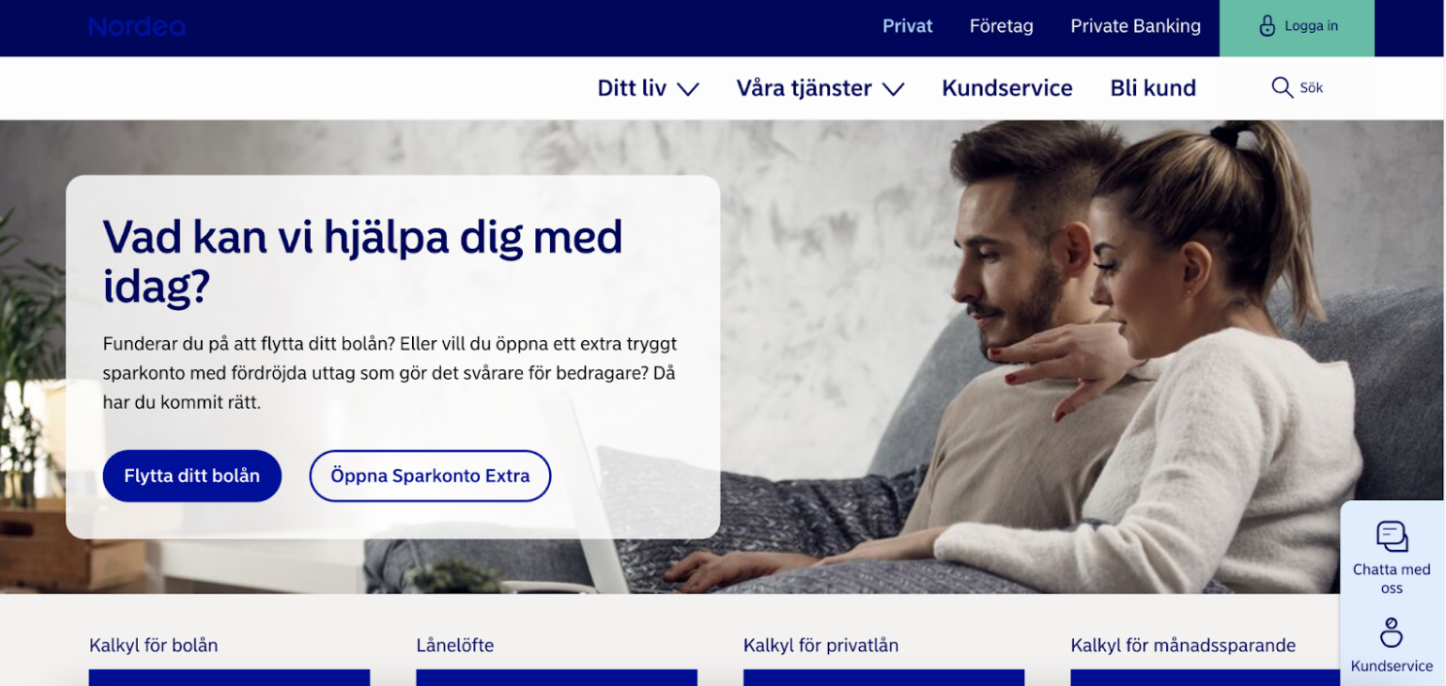
\includegraphics[width=\textwidth]{nordea.png}
\centering
\caption{Website nordea.se}
\label{screen:nordea}
\end{figure}

\noindent It’s worth noting that it’s IP address seen is the same internal one in the server, aka 192.168.1.201, indicating interaction with a cloned version of the website. Reconstruction of the page revealed differences from the original, indicating potential tampering. Screenshot \ref{screen:nordea} shows the original nordea webpage. On our reconstructed webpage, details wer missing, like pictures, graphics, etc. Out of the network traffic we were able to reconstruct the following timeline of events:
\begin{enumerate}
	\item User opened internetbanken.privat.nordea.se
	\item Request to get the IP Address of the DNS server was executed
	\item DNS server responded with a IP address corresponding to the record of \\internetbanken.privat.nordea.se (probably tampered DNS record)
	\item User accessed the IP address and arrived at a cloned version of the nordea website 
\end{enumerate}

\section{Discussion}
The analysis of the provided packet capture files (A.pcap, B.pcap, and C.pcap) revealed several noteworthy findings regarding suspicious wireless traffic in the small business environment, particularly concerning potential security threats and unauthorized activities.
\newline

\noindent In File \texttt{A.pcap}, the examination of WLAN traffic identified the network with the most activity. Although no specific encryption details were found in probe packets, the presence of WEP parameters in data packets suggested the possibility of WEP encryption. Through the use of the "aircrack-ng" tool, a WEP key "44:53:49:4C:41" was extracted, enabling decryption of all traffic for the SSID "DSI DSV." The analysis also highlighted IP communications involving private IP addresses 192.168.1.201 and external IP addresses 173.199.116.22 (The Constant Company LLC, US) and 74.125.15.84 (Google).
\newline

\noindent Moving on to File \texttt{B.pcap}, volumetric anomalies indicated a SYN flood attack, a form of Distributed Denial of Service (DDoS) attack. Additionally, repeated attempts to connect to various ports on the same targets using SYN packets indicated port scanning activity, a common reconnaissance tactic used by attackers.
\newline

\noindent Moving to File \texttt{C.pcap}, the client attempted to visit various websites, including "nordea.se," which responded back. Notably, the IP address seen was the same internal one on the server (192.168.1.201), indicating interaction with a cloned version of the website. Reconstruction of the webpage revealed differences from the original, indicating potential tampering. The timeline of events reconstructed from network traffic suggested DNS tampering, leading the user to access a cloned version of the Nordea website and therefore the potential leak of the banking information of the user.
\newline

\noindent In conclusion, based on the findings, it is evident that the small business network was subjected to various security threats and unauthorized activities. The presence of WEP encryption and indications of SYN flood attacks and port scanning activity suggest deliberate attempts to compromise the network's security. Furthermore, the reconstruction of the cloned Nordea website and DNS tampering point towards potential phishing or spoofing attempts aimed at obtaining sensitive information from users.